\section{Phân tích và tiền xử lý dữ liệu}

\subsection{Bộ dữ liệu: FoodSeg103}
FoodSeg103 là một trong những bộ dữ liệu chuẩn mực quy mô lớn đầu tiên được thiết kế chuyên biệt cho bài toán phân vùng hình ảnh thức ăn ở cấp độ nguyên liệu. Bộ dữ liệu này được giới thiệu bởi Wu và cộng sự tại hội nghị ACM Multimedia 2021, thông qua việc chắt lọc và gán nhãn thủ công từ Recipe1M - một kho dữ liệu khổng lồ chứa hàng triệu hình ảnh và công thức nấu ăn. Khác với các bộ dữ liệu trước đây thường chỉ giải quyết bài toán phân loại vùng có món ăn, FoodSeg103 đi sâu vào chi tiết của từng thành phần nguyên liệu cấu tạo nên món ăn đó.

Tập dữ liệu gồm tổng cộng 6117 ảnh, trong đó có 3982 ảnh huấn luyện và 2135 ảnh kiểm thử. Kích thước ảnh trung bình của train là $770.80\times640.58$ pixel, lớn hơn đáng kể so với test ở mức $578.80\times480.01$ pixel. Sự khác biệt về kích thước này dễ dẫn đến hiện tượng \emph{domain gap} do độ phân giải, làm suy giảm độ tin cậy của mô hình nếu dữ liệu không được tiền xử lý và chuẩn hóa nhất quán trên cả hai tập (split).

Về độ toàn vẹn, bộ dữ liệu đạt chất lượng gần như tuyệt đối với tỷ lệ ảnh hợp lệ trên 99.97\% ở cả hai tập và bao phủ đầy đủ toàn bộ 103 lớp foreground được định nghĩa trong metadata.

\begin{table}[H]
    \centering
    \caption{Toàn vẹn dữ liệu trên bộ dữ liệu gốc}
    \begin{tabular}{lrrr}
        \toprule
        Split & Ảnh hợp lệ & Tổng ảnh & Tỉ lệ hợp lệ \\
        \midrule
        Train & 3981 & 3982 & 99.97\% \\
        Test  & 2135 & 2135 & 100.00\% \\
        \bottomrule
    \end{tabular}
\end{table}

Vấn đề đáng chú ý nhất của bộ dữ liệu là sự phân bố đuôi dài nghiêm trọng. Theo thống kê mức bao phủ pixel, các lớp phổ biến như \texttt{chicken duck} và \texttt{bread} chiếm lần lượt 4.91\% và 3.34\% tổng số pixel, trong khi các lớp hiếm như \texttt{bamboo shoots} và \texttt{kelp} gần như bằng 0 (xấp xỉ 0.0004\%). Về mặt vật thể, nhóm phổ biến xuất hiện hơn 1100 lần, bỏ xa các lớp còn lại. Do đó, nếu không có chiến lược tái cấu trúc không gian nhãn, mô hình sẽ rơi vào trạng thái thiên lệch, chỉ tối ưu hóa tốt cho nhóm chiếm đa số nhưng lại thất bại trong việc phân vùng nhóm thiểu số.

\begin{figure}[H]
    \centering
    \begin{subfigure}[t]{0.49\linewidth}
        \centering
        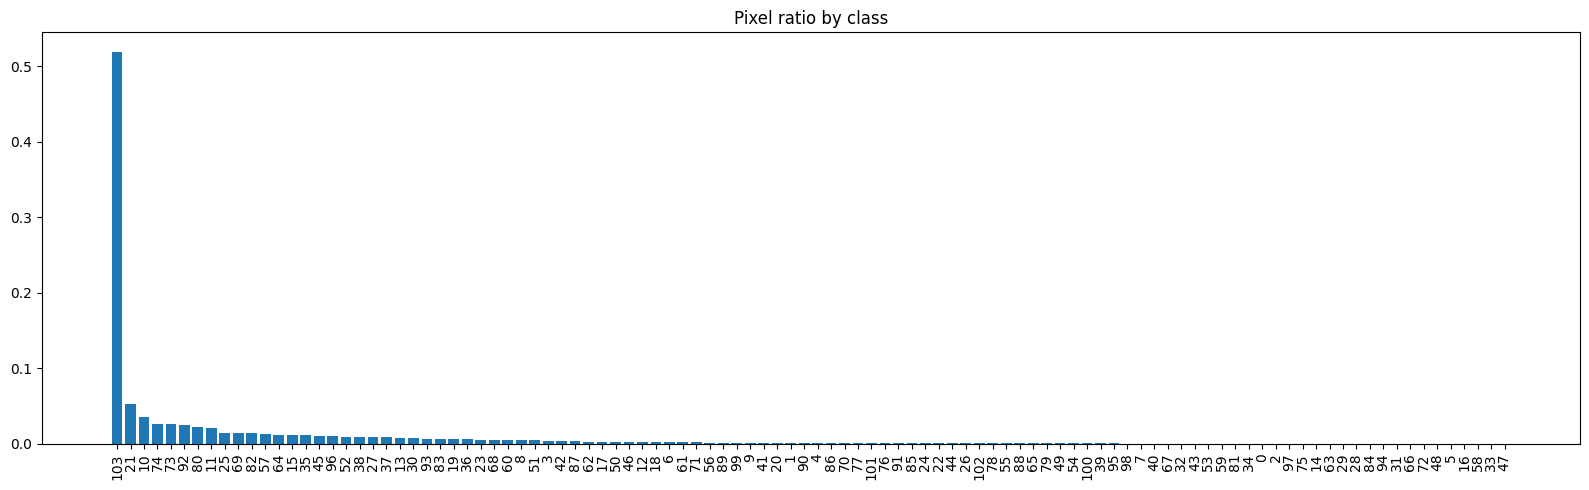
\includegraphics[width=\linewidth]{img/analyze/pixel-ratio-by-class.png}
        \caption{Tỉ lệ pixel theo từng lớp}
    \end{subfigure}
    \hfill
    \begin{subfigure}[t]{0.49\linewidth}
        \centering
        
\includegraphics[width=\linewidth]{img/analyze/image-presence-ratio-by-class.png}
        \caption{Tỉ lệ ảnh có xuất hiện từng lớp}
    \end{subfigure}
    \caption{Biểu hiện mất cân bằng lớp trên FoodSeg103 gốc theo mức bao phủ pixel và tần suất xuất hiện theo ảnh.}
\end{figure}

\subsection{Quy trình cân bằng lại dữ liệu}
Quy trình tái cấu trúc dữ liệu trên bộ dữ liệu FoodSeg103 nhằm giảm độ phân mảnh nhãn đồng thời giữ nguyên giá trị ngữ nghĩa cốt lõi. Chiến lược chính là gộp nhãn theo ngữ nghĩa, đặc biệt chú trọng đến độ tương đồng giữa các lớp con trước khi gộp.

Cụ thể, các nhóm lớp được gộp lại khi chúng chia sẻ đặc trưng thống nhất: ví dụ, các loại nấm khác nhau được gộp thành mushroom nhờ cách thức chế biến giống nhau, thành ra có sự tương đồng về màu sắc và vân.

\begin{table}[htbp]
\centering
\caption{Các nhóm lớp được gộp theo ngữ nghĩa và đặc trưng kết cấu bề mặt}
\label{tab:merge_groups}
\begin{tabular}{p{0.5\linewidth}p{0.29\linewidth}}
\toprule
\textbf{Nhóm lớp gốc} & \textbf{Lớp đích sau khi gộp} \\
\midrule
king oyster mushroom, oyster mushroom, enoki mushroom, white button mushroom, shiitake) 
& \texttt{mushroom} \\
\midrule
green beans, french beans, snow peas, bean sprouts, soy, red beans, okra 
& \texttt{beans\_and\_peas} \\
\midrule
peanut, almond, cashew, walnut 
& \texttt{nut} \\
\midrule
cake, biscuit, pudding, egg tart, candy, chocolate, popcorn 
& \texttt{desserts} \\
\midrule
lemon, orange 
& \texttt{citrus} \\
\midrule
spring onion, onion, garlic, ginger 
& \texttt{alliums\_and\_garlic} \\
\midrule
cabbage, rape, lettuce 
& \texttt{leafy\_greens} \\
\midrule
kelp, seaweed
& \texttt{seaweed} \\
\bottomrule
\end{tabular}
\end{table}

Các lớp có tần suất rất thấp hoặc không đủ đặc trưng vân/màu sắc để giữ riêng sẽ được ánh xạ vào các lớp bao quát \texttt{other ingredients}. Cách tiếp cận này không chỉ giảm số lớp từ 103 xuống còn 75 mà còn tăng đáng kể kích thước mẫu huấn luyện hiệu quả cho từng lớp đích, hạn chế mất mát thông tin so với việc drop hoàn toàn.

\
\subsection{Dữ liệu sau xử lý}

Không gian nhãn giảm từ 103 xuống 75 lớp. Về số lượng ảnh, tập train giảm từ 3982 xuống 3981 ảnh (giảm 1 ảnh) và tập test giữ nguyên 2135 ảnh. Theo thống kê export trong notebook, ảnh bị loại chủ yếu do lỗi hỏng tệp ảnh (bad image), trong khi số ảnh bị loại do empty mask sau ánh xạ là 0 ở cả hai split.

\begin{table}[H]
    \centering
    \caption{So sánh dữ liệu trước và sau xử lý}
    \begin{tabular}{lrr}
        \toprule
        Chỉ số & Trước xử lý & Sau xử lý \\
        \midrule
        Số lớp mục tiêu & 103 & 75 \\
        Số ảnh train & 3982 & 3981 \\
        Số ảnh test & 2135 & 2135 \\
        \bottomrule
    \end{tabular}
\end{table}

Từ góc nhìn huấn luyện, bộ \texttt{FoodSeg103\_rebalanced} giúp giảm áp lực học trên các lớp cực hiếm và tăng tính ổn định của tối ưu hóa. Tuy nhiên, long-tail chưa biến mất hoàn toàn, nên các kỹ thuật như \emph{focal loss}, \emph{class-weighted loss}, cùng theo dõi \emph{per-class IoU} vẫn là cần thiết để bảo đảm mô hình không thiên lệch về lớp đa số.